\chapter{Objetivos y motivación}


\bigskip
Un algoritmo es una serie de pasos organizados que describe el proceso que se debe seguir, para dar solución a un problema específico. A principios de la década de 1960, en 1962 John Henry Holland ideó una de las líneas más prometedoras de la inteligencia artificial, la de los algoritmos genéticos, y con su libro ``Adaptation in Natural and Artifical Systems`` en 1975 logró una mayor popularidad. 

Estos algoritmos son llamados así porque se inspiran en la evolución biológica y su base genético-molecular. Estos algoritmos hacen evolucionar una población de individuos sometiéndola a acciones aleatorias semejantes a las que actúan en la evolución biológica (mutaciones y recombinaciones genéticas), así como también a una selección de acuerdo con algún criterio, en función del cual se decide cuáles son los individuos más adaptados, que sobreviven, y cuáles los menos aptos, que son descartados.

\bigskip
Para su funcionamiento (el de un algoritmo genético simple, llamado Canónico), al empezar necesita una codificación o representación del problema que se adecue al mismo y una función de ajuste o adaptación al problema. Durante la ejecución del algoritmo, se seleccionan unos individuos para cruzarlos, y  al individuo que resulte de este cruce se le hará una mutación. El resultado será un conjunto de individuos (posibles soluciones al problema) que formarán parte de la siguiente población. El algoritmo repetirá el proceso hasta encontrar una solución óptima o las veces que se le indique.

\bigskip
Poseen multitud de aplicaciones, como pueden ser:

\begin{itemize}
	\item Diseño automatizado para la investigación de diseño de materiales \cite{5586262}, equipamiento industrial o sistemas de comercio en el sector financiero.
	\item Construcción de árboles filogenéticos. \cite{arbolesfilogeneticos}
	\item Diseño de sistemas de distribución de aguas \cite{ditribucionagua}. 
	\item Resolución de equilibrios en Teoría de juegos \cite{teoriajuegos}.
	\item Análisis de expresión de genes \cite{analisisexpresiongenes}.
\end{itemize}

\bigskip
Pueden resolver problemas de alta complejidad, pero esto suele traducirse en operaciones muy costosas en términos de tiempo y recursos. En la actualidad, por ejemplo, hay casos en los que recrear una simulación de la solución propuesta por una iteración puede durar varios días y consumir gran cantidad de procesamiento y recursos asociados.


\bigskip
Estos algoritmos consumen muchos recursos y estos recursos no siempre están disponibles o al alcance de todo el mundo. Por esta razón, este proyecto Fin de Máster propone hacer accesible recursos de computación de bajo coste y alta disponibilidad a usuarios que no tienen la posibilidad de pagar dicho servicio o que no los tienen disponibles en su máquina. Estos recursos de computación son las tarjetas gráficas programables o GPU \cite{gpgpu}. Las GPUs ponen a disposición de los usuarios un recurso de computación paralelo muy potente a un precio no muy elevado y están siendo en los últimos años una tendencia en la paralelización de los algoritmos genéticos. Esta tendencia permite el desarrollo de este trabajo Fin de Máster estableciendo un primer paso en el desarrollo de servicios web que permitan acceder a estos recursos y que puedan estar instalados en cualquier máquina de esta escuela, facilitando el acceso a los alumnos a estos recursos sin necesidad de estar presentes en las aulas.



\bigskip
\section{Objetivos}
\bigskip


\begin{itemize}
	
	\item  Desarrollar el conjunto de clases que permita acceder de forma remota a un conjunto de recursos para la ejecución de algoritmos evolutivos paralelos.
	\item  Acceder a un recurso de computación remoto a través de un interfaz web.
	\item  Aprender a utilizar recursos de computación paralela de bajo coste como son las GPUs
	\item  Estudiar el rendimiento obtenido para esta interfaz web en comparación con otras alternativas.
	
\end{itemize}



\bigskip
\section{Motivación}
\bigskip

Dicha complejidad en la resolución de los algoritmos genéticos lleva a optimizarlos y a trabajar con ellos para lograr reducir el coste de dichas operaciones. 

Esto lleva a utilizar una computación paralela, en la que se aprovecha la potencia de computación de los sistemas con los que trabajamos realizando cálculos simultáneamente. Sigue el principio de dividir los problemas grandes en problemas más pequeños, que se solucionan en paralelo para luego obtener la solución del problema inicial.

Por otra parte, en el ámbito de la computación se ha visto una gran evolución de las tarjetas gráficas, ya que grandes fabricantes como NVIDIA, AMD, IBM o Intel han logrado una producción de GPUs de gran alcance, como se puede ver en la Figura \ref{fig:gpu_vs_cpu} (pueden incluso superar la frecuencia de reloj de una CPU antigua).

\bigskip
\begin{figure}[h]
	\centering
	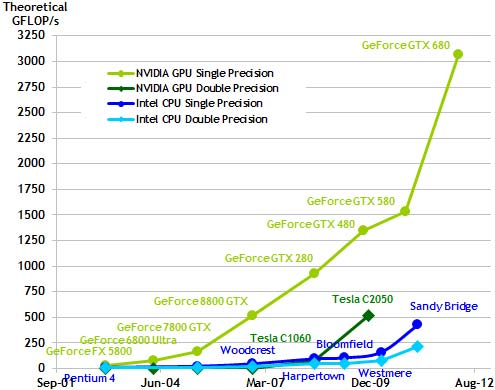
\includegraphics[width=0.7\linewidth]{../images/gpu_vs_cpu}
	\caption[Evolución de las GPUs respecto a las CPUs]{Evolución hasta 2012 de las GPUs respecto a las CPUs}
	\label{fig:gpu_vs_cpu}
\end{figure}


\bigskip
El uso de computación paralela, junto la potencia y la posibilidad de usar el paralelismo que ofrecen las GPU  hace muy interesante el uso de dichas GPUs para resolver algoritmos genéticos de formas más eficiente.

Después del estudio realizado en el siguiente capítulo, se opta por usar la arquitectura de cálculo CUDA \cite{nvidiacuda} para crear algoritmos genéticos que se ejecuten en GPUs de NVIDIA \cite{nvidiadeveloper}.

Como se cita en uno de los objetivos, se publicará de manera que cualquier usuario tenga acceso. Esto, junto a una interfaz sencilla, permitirá computar algoritmos genéticos con facilidad y rapidez.




